\documentclass[conference]{IEEEtran}
\usepackage[T1]{fontenc} % Use 8-bit encoding that has 256 glyphs
\usepackage{fourier} % Use the Adobe Utopia font for the document - comment this line to return to the LaTeX default
\usepackage[english]{babel} % English language/hyphenation
\usepackage{amsmath,amsfonts,amsthm} % Math packages
\usepackage{graphicx}
\usepackage{lipsum} % Used for inserting dummy 'Lorem ipsum' text into the template
\usepackage{tikz}
\usetikzlibrary{fit,shapes}
\usetikzlibrary{arrows,positioning}
\tikzset{
    %Define standard arrow tip
    >=stealth',
    %Define style for boxes
    punkt/.style={
           rectangle,
           rounded corners,
           draw=black, very thick,
           text width=6.5em,
           minimum height=2em,
           text centered},
    % Define arrow style
    pil/.style={
           ->,
           thick,
           shorten <=2pt,
           shorten >=2pt,}
}


\hyphenation{op-tical net-works semi-conduc-tor}
\begin{document}
\title{An Extended Kalman Filter for Real-Time Estimation and Control of a
Rigid-Link Flexible-Joint Manipulator}
\author{\IEEEauthorblockN{Mahyar Abdeetedal}
\IEEEauthorblockA{Department of Electrical and\\Computer Engineering\\
University of Western Ontario\\
London, ON, Canada\\
Email: mabdeete@uwo.ca}} 
\maketitle


\begin{abstract}
High performance tracking of an industrial robot depends on accurate expression
of manipulator dynamics. When a robot has flexible joints efficient model
parametrization will be difficult to achieve. In this course project report an
extended Kalman filter (EKF) observer to estimate manipulator states is
presented. In a computer simulation the estimation performance is demonstrated.
Experimental setup for KUKA/DLR Light-Weight robot is also introduced. Lagrangian
method is used for robot modeling and all maple files are included on github.
\end{abstract}
\IEEEpeerreviewmaketitle



\section{Introduction}
In industrial robots, the presence of transmission elements such as harmonic
drives and transmission belts (typically, Scara arms) long shafts (e.g., last
3-dofs of Puma) introduce flexibility effects between actuating inputs and
driven outputs (Fig. \ref{2robot}). In the flexible joint model, not only the
motor position $q$, but also the joint torque $\tau$, as well as their derivatives $\dot{q}$ and
$\dot{\tau}$  are namely states of the system. The measurement of the former and
the numerical computation of the latter provides the state estimation required
for full state feedback. For the light-weight arm and hands, these methods were
presented, e.g., in \cite{1}, \cite{2}, \cite{3}, and \cite{4}.

Taking into account the elasticity of the transmission, each joint becomes a
mass-spring-damper system (Fig. \ref{flexiblejoint}) (and thus a fourth order
system), so that the complete state is given by position and velocity (as for the second
order rigid robot model), and additionally by the torque and its derivative.


\begin{figure}
\begin{center}
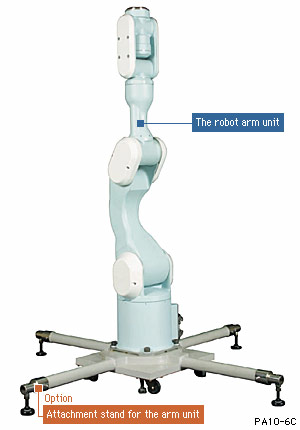
\includegraphics[width=.2\textwidth]{pa10.jpg}
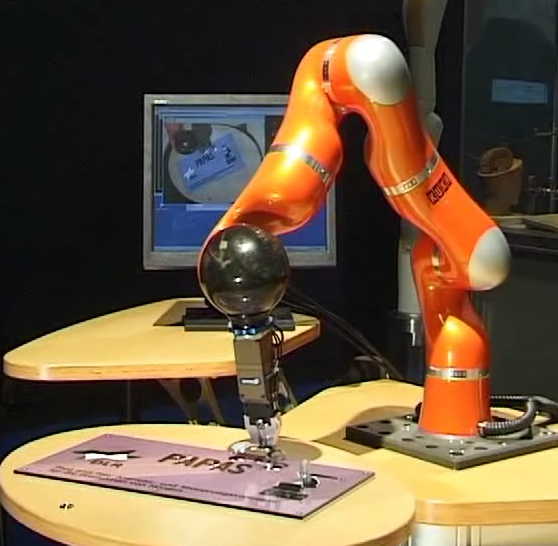
\includegraphics[width=.2\textwidth]{kuka.png}
\end{center}
\caption{Mitsubishi PA10 arm and KUKA light-weight arm}
\label{2robot}
\end{figure}

\begin{figure}
\centering
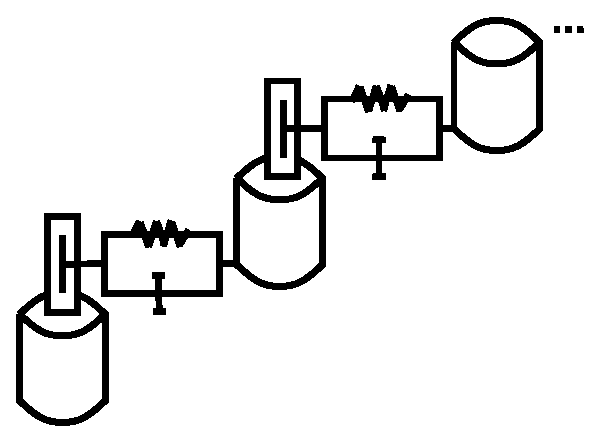
\includegraphics[width=.2 \textwidth]{flexibleJointRobot.eps}
\caption{Flexible joint rigid link robot.}
\label{flexiblejoint} 
\end{figure}
  

In the paper which is chosen for this course \cite{article}, an EKF is proposed
to estimate link and motor positions/velocities in a Rigid Link Flexible Joint
(RLFJ) manipulator. The main contribution of this article is the design and
implementation of a new observer-controller combination for accurate estimation
and control of a RLFJ manipulator. The state vector in this work contains link
and motor positions/velocities, unknown dynamic and kinematic parameter
estimates, and link positions.

In this report main focus is on the observer design rather than the
contributions on manipulator control approach. The adaptive RLFJ controller
utilizes EKF-based estimates of link and motor positions/velocities.

This report is organised into six sections. Sections II and III outline the
design of the EKF observer and its corresponding RLFJ controller. Section IV
describes the simulation model and results. Section V details the experimental
setup, procedure, and results. Section VI provides conclusions of the results.

\section{Extended Kalman Filter Observer}

\subsection{Rigid-Link Flexible-Joint Model}
The $n$-link rigid-link flexible-joint (RLFJ) robot dynamics can be expressed as

\begin{equation}
\begin{array}{ccccc}
M(q)\ddot q + {V_m}(q,\dot q)\dot q + G(q) + {F_L}(\dot q) + {K_S}(q - {q_m}) = 0\\
J{{\ddot q}_m} + B{{\dot q}_m} + {K_S}({q_m} - q) = u
\end{array}
\label{1}
\end{equation}

where $q(t),\dot q(t),\ddot q(t) \in {R^n}$ and ${q_m}(t),{{\dot
q}_m}(t),{{\ddot q}_m}(t) \in {R^n}$ are the position, velocity, and
acceleration of the link and motor angles, respectively, $M(q) \in {R^{n \times
n}}$ is inertia matrix, ${V_m}(q,\dot q) \in {R^{n \times n}}$ is
centripetal-Coriolis matrix, $G(q) \in {R^n}$ and ${F_L}(\dot q) \in {R^n}$ are
the gravitational and frictional effects of the link dynamics, respectively,
${K_S}$, $J$, and $B \in {R^n}$ are constant, diagonal, positive-definite
matrices representing joint stiffness, motor inertia, and motor viscous
friction, respectively, and $u(t) \in {R^n}$ is the motor torque. There are also
unknown and varying parameters in the dynamic model of the robot which can be
shown by $\theta  \in {R^p}$.

Sets of retro-reflective markers can be attached to the surface of the robot to
improve the accuracy of the link position measurement. The position of the $i$th
marker in link coordinate system $L_i$ can be identified as $p_i^{{L_i}}$,
with $i = 1,\ldots,m$, and the collection of all markers in their respective
local coordinate systems as ${p^L} \in {R^{3m}}$. Let us also define a
kinematic parameter vector $\phi  \in {R^6}$ to represent the position and
orientation of the robot coordinate system in the motion capture coordinate
system. The the state vector can be defined as

\begin{equation}
x = {[\begin{array}{*{20}{c}}
{{q^T}}&{{{\dot q}^T}}&{q_m^T}&{\dot q_m^T}&{{\theta ^T}}&{{\phi ^T}}&{{{({p^L})}^T}}
\end{array}]^T}
\label{4}
\end{equation}

such that $\dot x = f(x,u)$ where

\begin{equation}
f(x,u) = \left[ {\begin{array}{*{20}{c}}
{\dot q}\\
{\ddot q = {M^{ - 1}}(q,\theta )({K_S}({q_m} - q) - {V_m}(q,\dot q,\theta )\dot q - G(q,\theta ) - {F_L}(\dot q,\theta ))}\\
{{{\dot q}_m}}\\
{{J^{ - 1}}(u - B{{\dot q}_m} - {K_S}({q_m} - q))}\\
0
\end{array}} \right]
\label{5}
\end{equation}

The random vaiable regarding the uncertainties can be grouped as $\omega  =
{[\begin{array}{*{20}{c}} {\omega _L^T}&{\omega _M^T}&{\omega _\theta ^T}&{\omega _\phi ^T}&{\omega _P^T}
\end{array}]^T}$ where ${\omega _L}$ and ${\omega _M}$ are random variables
related to uncertainties in the link and motor dynamics respectively. The
unknown dynamic and kinematic parameter estimates are modeled as random walk
processes, such that $\dot \theta  = {\omega _\theta }$, $\dot \phi  = {\omega _\phi }$, and ${{\dot p}^L}
= {\omega _P}$. we can write

\begin{equation}
\dot x = f(x,u) + G(x)\omega
\label{6}
\end{equation}

\begin{equation}
G(x) = \left[ {\begin{array}{*{20}{c}}
0&0&0&0&0\\
{{M^{ - 1}}(q,\theta )}&0&0&0&0\\
0&0&0&0&0\\
0&{{J^{ - 1}}}&0&0&0\\
0&0&{{I_{Param}}}&0&0\\
0&0&0&{{I_{Trans}}}&0\\
0&0&0&0&{{I_{Geom}}}
\end{array}} \right]
\label{7}
\end{equation}


and its first-order Taylor expansion is

\begin{equation}
{{\dot x}_0} = f({x_0},{u_0})
\label{8}
\end{equation}

\begin{equation}
\delta \dot x = \frac{{\partial f(x,u)}}{{\partial x}}\delta x +
G({x_0})\omega  + \varphi (x,{x_0},{u_0})
\label{9}
\end{equation}

where $\varphi (x,{x_0},{u_0})$ is the higher order terms. and

\begin{equation}
\begin{array}{ccccc}
\frac{{\partial f}}{{\partial x}} = F(t) = \left[ {\begin{array}{*{20}{c}}
0&I&0&0&0&0&0\\
{{F_{21}}}&{{F_{22}}}&{{F_{23}}}&0&{{F_{25}}}&0&0\\
0&0&0&I&0&0&0\\
{{F_{41}}}&0&{{F_{43}}}&{{F_{44}}}&{{F_{45}}}&0&0\\
0&0&0&0&0&0&0
\end{array}} \right]\\
{F_{21}} =  - {M^{ - 1}}(\frac{{\partial M}}{{\partial q}}\ddot q + \frac{{\partial {V_m}}}{{\partial q}}\dot q + \frac{{\partial G}}{{\partial q}} + {K_S})\\
{F_{22}} =  - {M^{ - 1}}(\frac{{\partial {V_m}}}{{\partial \dot q}}\dot q + {V_m} + \frac{{\partial {F_L}}}{{\partial \dot q}})\\
{F_{23}} = {M^{ - 1}}K\\
{F_{25}} =  - {M^{ - 1}}(\frac{{\partial M}}{{\partial \theta }}\ddot q + \frac{{\partial {V_m}}}{{\partial \theta }}\dot q + \frac{{\partial G}}{{\partial \theta }} + \frac{{\partial {F_L}}}{{\partial \theta }} + \frac{{\partial {K_S}}}{{\partial \theta }}(q - {q_m}))\\
{F_{41}} = {J^{ - 1}}{K_S}\\
{F_{43}} =  - {J^{ - 1}}{K_S}\\
{F_{44}} =  - {J^{ - 1}}B\\
{F_{45}} =  - {J^{ - 1}}(\frac{{\partial J}}{{\partial \theta }}{{\ddot q}_m} + \frac{{\partial B}}{{\partial \theta }}{{\dot q}_m} + \frac{{\partial {K_S}}}{{\partial \theta }}({q_m} - q))
\end{array}
\label{10}
\end{equation}

\subsection{Measurement Model}
Measurement vector can be defined as


\begin{equation}
h(x) = {[\begin{array}{*{20}{c}}
{q_m^T}&{\dot q_m^T}&{{{({p^G})}^T}}
\end{array}]^T}
\label{12}
\end{equation}

where ${p^G}(q,\phi ,{p^L}) \in {R^{3m}}$ is the position of all markers on the
links in the global coordinate system. We can consider the vector $v =
{[\begin{array}{*{20}{c}} {v_1^T}&{v_2^T}&{v_3^T}
\end{array}]^T}$ as random variable, such that

\begin{equation}
y = h(x) + v
\label{13}
\end{equation}

We can also write

\begin{equation}
{y_0} = h({x_0})
\label{14}
\end{equation}

\begin{equation}
\delta y = \frac{{\partial h({x_0})}}{{\partial x}}\delta x + v + \xi
(x,{x_0})
\label{15}
\end{equation}

where $\xi (x,{x_0})$ is the higher order terms. and

\begin{equation}
\begin{array}{l}
\frac{{\partial h}}{{\partial x}} = H(t) = \left[ {\begin{array}{*{20}{c}}
0&0&I&0&0&0&0\\
0&0&0&I&0&0&0\\
{{H_{31}}}&0&0&0&0&{{H_{36}}}&{{H_{37}}}
\end{array}} \right]\\
{H_{31}} = \left[ {\begin{array}{*{20}{c}}
{{{\frac{{\partial p_1^G}}{{\partial q}}}^T}}& \cdots &{{{\frac{{\partial p_M^G}}{{\partial q}}}^T}}
\end{array}} \right]\\
{H_{36}} = \left[ {\begin{array}{*{20}{c}}
{{{\frac{{\partial p_1^G}}{{\partial \phi }}}^T}}& \cdots &{{{\frac{{\partial p_M^G}}{{\partial \phi }}}^T}}
\end{array}} \right]\\
{H_{37}} = \left[ {\begin{array}{*{20}{c}}
{{{\frac{{\partial p_1^G}}{{\partial p_1^{{L_1}}}}}^T}}&0&0\\
0& \ddots &0\\
0&0&{{{\frac{{\partial p_1^G}}{{\partial p_M^{{L_M}}}}}^T}}
\end{array}} \right]
\end{array}
\label{16}
\end{equation}


\subsection{Continuous-Time Extended Kalman Filter}
In the reviewed paper \cite{article}, it attempts a slight modification of the
extended Kalman filter to adjust the dynamics with an aim of increasing the
domain of attraction and reducing the time for error decay. The basic method
consists of determining the observer gain for a fictitious more instable
system. This is done by supplying the system matrix, which is set-up by a
standard linearisation, with an additive unstable term. For the case of linear
stochastic systems the design is known as exponential data weighting. 

Given the system and measurement models in (\ref{6}) and (\ref{13}), having
zero-mean Gaussian noise covariance matrices $Q(t)$ and $R(t)$, the state
estimate and error covariance update equations are
\begin{equation}
\dot \hat x = f(\hat x,u) + K(t)[y(t) - h(\hat x)]
\label{22}
\end{equation}

\begin{equation}
\begin{array}{l}
\dot P(t) = (F(\hat x,t) + \alpha {I_n})P(t) + P(t){(F(\hat x,t) + \alpha {I_n})^T}\\
 + G(\hat x,t)Q(t){G^T}(\hat x,t) - K(t)H(t)P(t)
\end{array}
\label{23}
\end{equation}

with $\alpha > 0$ and the Kalman gain $K(t)=P(t)H^T(t)R^{-1}$.

There are three assumptions which must be satisfied in order to prove
exponential stability of the EKF which can be found in \cite{article}
and \cite{ar}.


\subsection{Discrete-Time Extended Kalman Filter}

The discrete-time EKF is an extension of the EKF to discrete-time systems. The
updated state estimate and error covariance matrix are obtained from the discrete-time EKF equations

\begin{equation}
x_k^ +  = x_k^ -  + {K_k}({z_k} - {H_k}x_k^ - )
\label{37}
\end{equation}

\begin{equation}
P_k^ +  = (I - {K_k}{H_k})P_k^ - ,
\label{38}
\end{equation}

\begin{equation}
{K_k} = P_k^ - H_k^T{({H_k}P_k^ - H_k^T + {R_k})^{ - 1}}
\label{39}
\end{equation}



\section{Controller}
Since the main focus of this report is on the state observer part not control
contributions readers are referred to part III of \cite{article} for details on
the proposed adaptive back-stepping controller.


\section{Simulation}
Simulations has been done for 2DOF planar robot (SCARA). Matrix $F$ which is the
partial derivative of the robot dynamics with respect to the states is
calculated for SCARA using maple. The maple file is attached to this report. 

Fig.(\ref{q1}), Fig.(\ref{q2}), Fig.(\ref{qdot1}), and Fig.(\ref{qdot2}) show
the estimation of $q_1$, $q_2$, $\dot q_1$, and $\dot q_2$ respectively.
Fig.(\ref{q1error}), Fig.(\ref{q2error}), Fig.(\ref{qdot1error}), and
Fig.(\ref{qdot2error}) show the error of estimation of $q_1$, $q_2$, $\dot q_1$,
and $\dot q_2$ respectively.

\begin{figure}
\centering
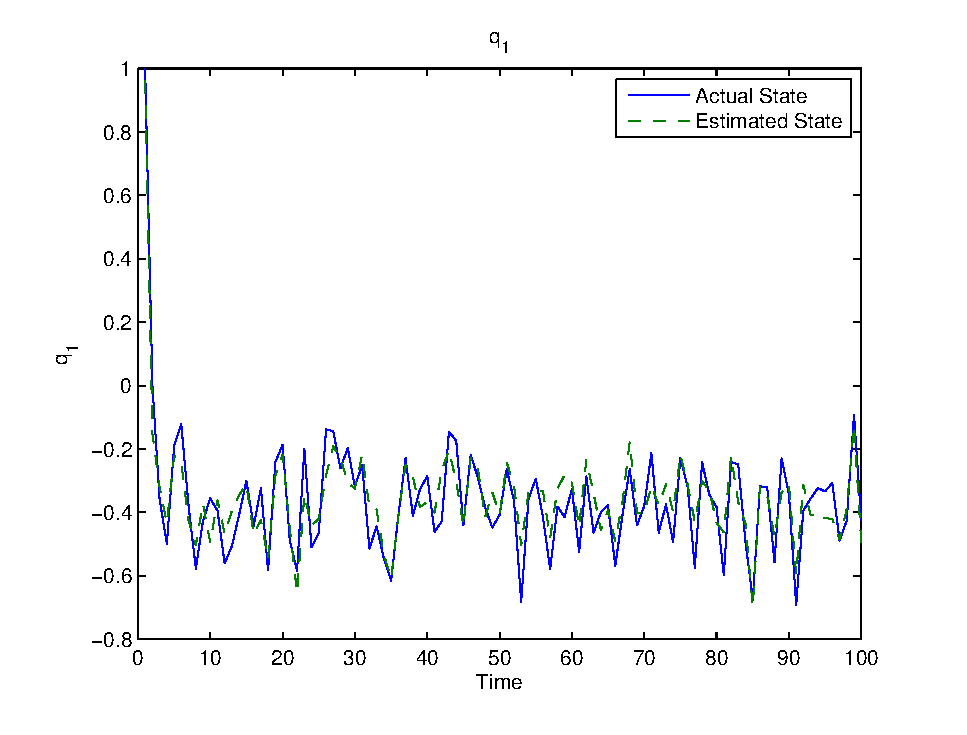
\includegraphics[width=.4 \textwidth]{q1.eps}
\caption{Estimation of $q_1$}
\label{q1}
\end{figure}

\begin{figure}
\centering
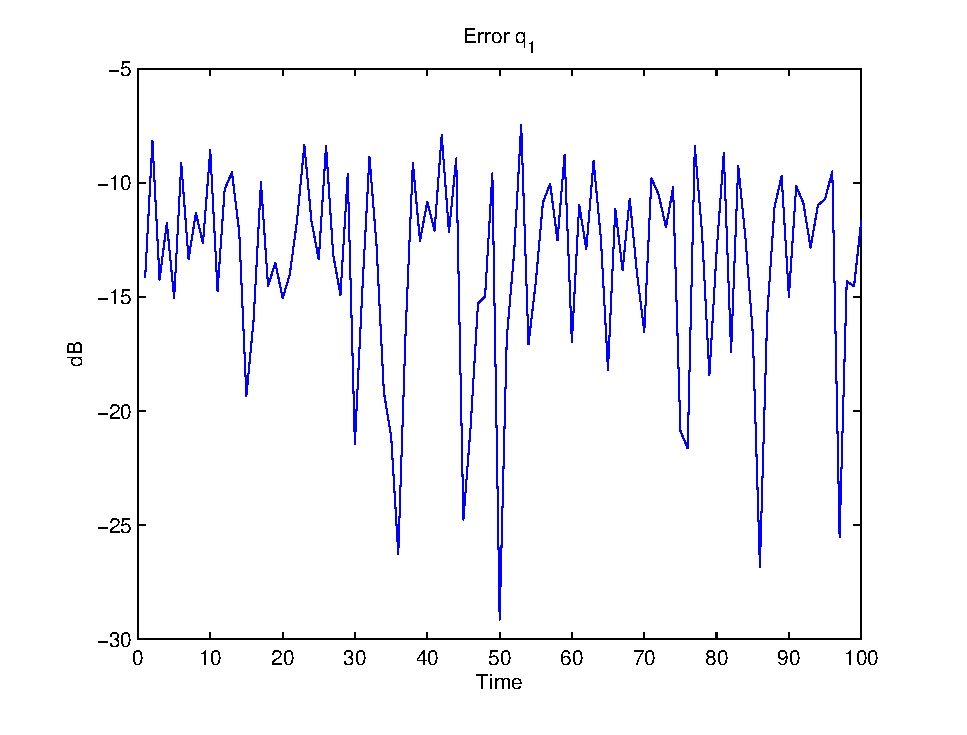
\includegraphics[width=.4 \textwidth]{q1error.eps}
\caption{Estimation error of $q_1$}
\label{q1error}
\end{figure}

\begin{figure}
\centering
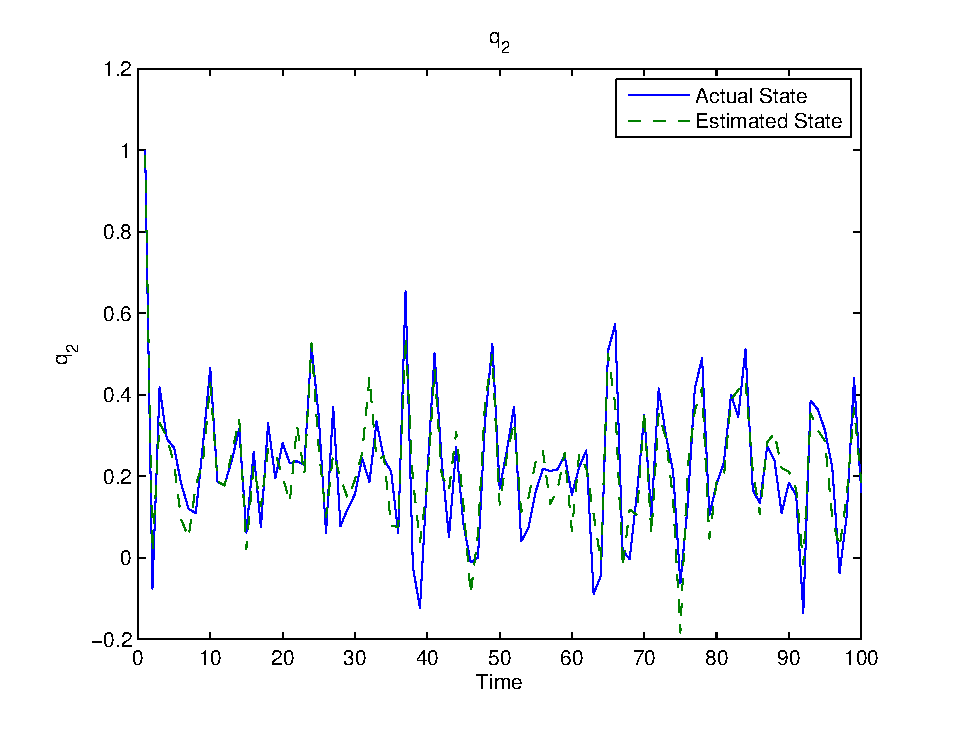
\includegraphics[width=.4 \textwidth]{q2.eps}
\caption{Estimation of $q_2$}
\label{q2}
\end{figure}

\begin{figure}
\centering
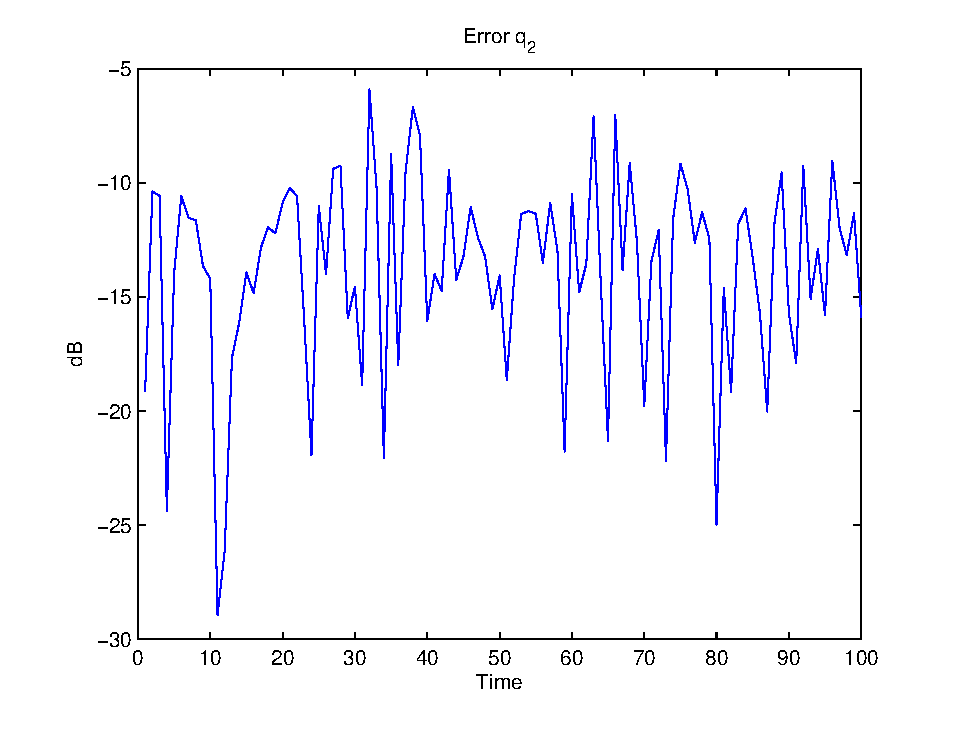
\includegraphics[width=.4 \textwidth]{q2error.eps}
\caption{Estimation error of $q_2$}
\label{q2error}
\end{figure}

\begin{figure}
\centering
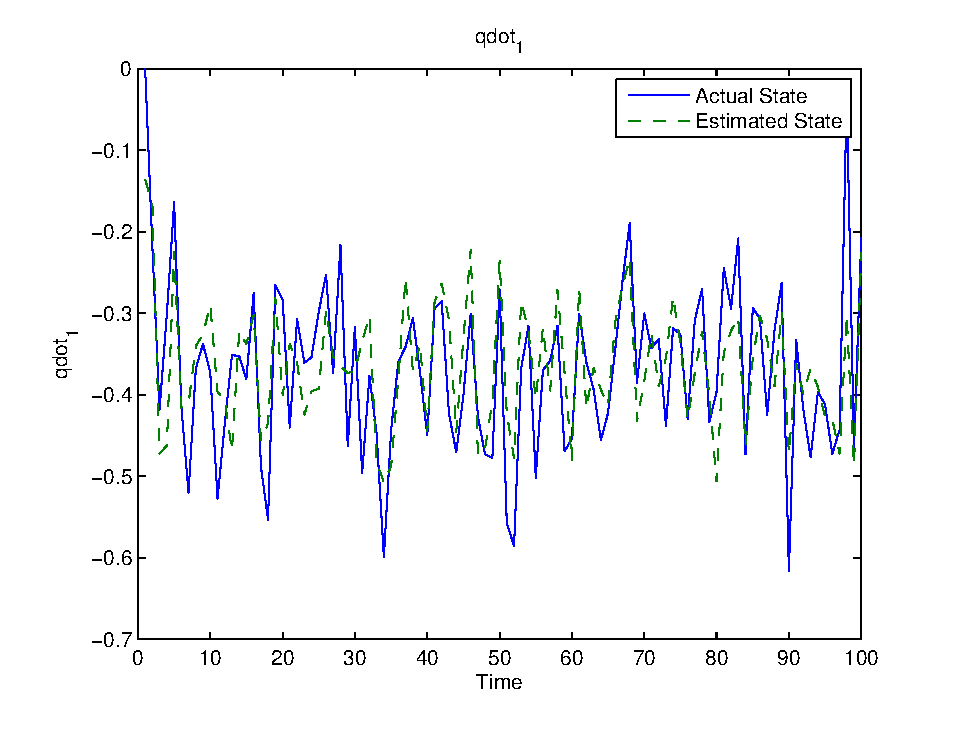
\includegraphics[width=.4 \textwidth]{qdot1.eps}
\caption{Estimation of $\dot{q_1}$}
\label{qdot1}
\end{figure}

\begin{figure}
\centering
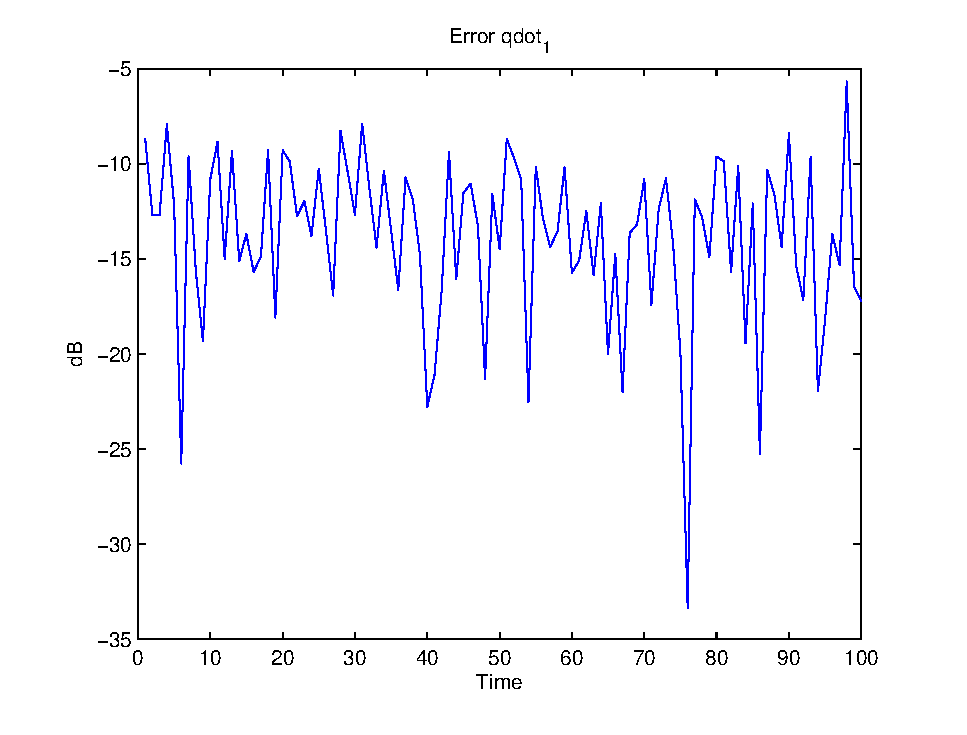
\includegraphics[width=.4 \textwidth]{qdot1error.eps}
\caption{Estimation error of $\dot{q_1}$}
\label{qdot1error}
\end{figure}

\begin{figure}
\centering
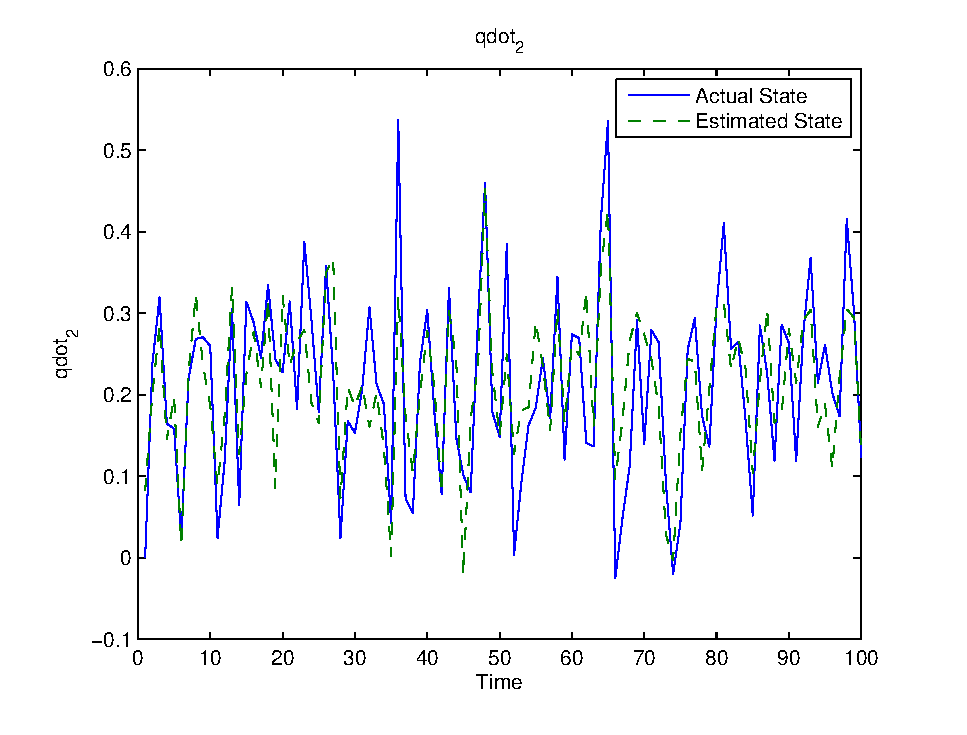
\includegraphics[width=.4 \textwidth]{qdot2.eps}
\caption{Estimation of $\dot{q_2}$}
\label{qdot2}
\end{figure}

\begin{figure}
\centering
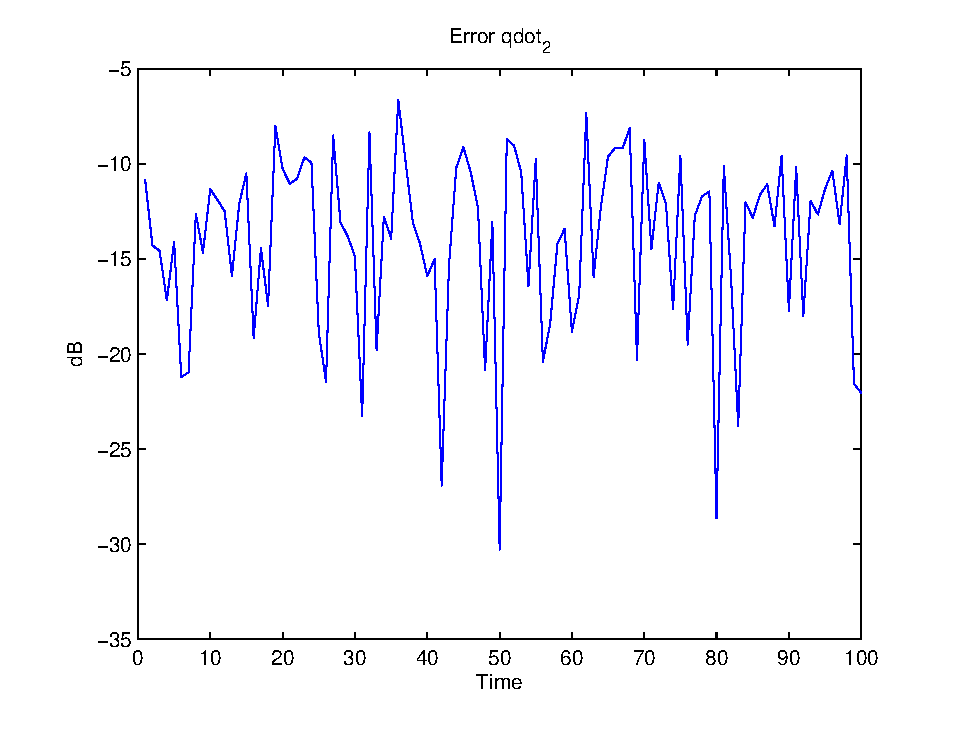
\includegraphics[width=.4 \textwidth]{qdot2error.eps}
\caption{Estimation error of $\dot{q_2}$}
\label{qdot2error}
\end{figure}
\section{Experiment}

\subsection{Experimental Setup}
DLR/KUKA Light Weight Robot III in Human Robot Interaction Lab. at the
University of Western Ontario is considered to be used as a test bed for the
proposed controller and state observer. This robot is shown in
Fig.\ref{kukasetup}.
\begin{figure}
\centering
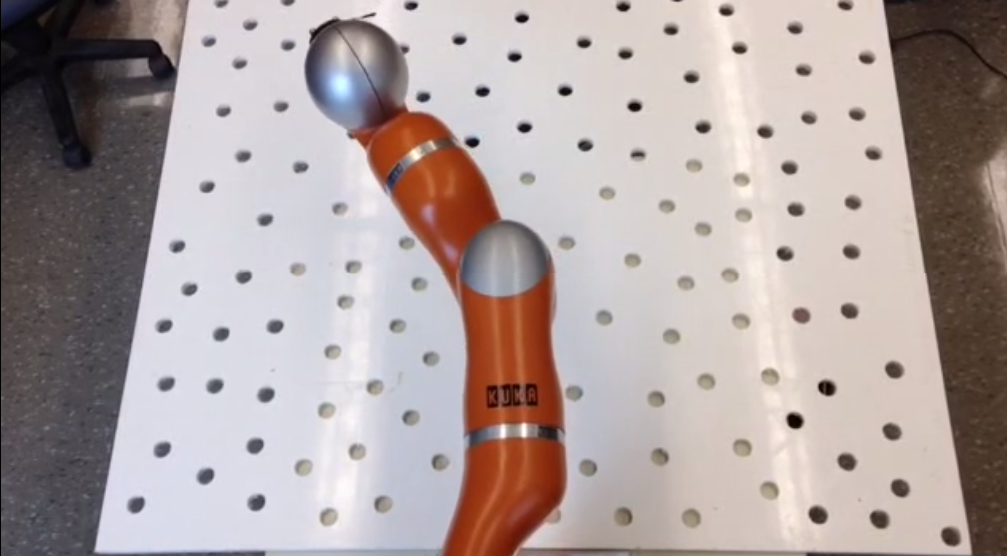
\includegraphics[width=.4 \textwidth]{experimentalSetup.png}
\caption{DLR/KUKA Light Weight Robot III, Human robot Interaction Lab.,
University of Western Ontario.}
\label{kukasetup}
\end{figure}

\subsection{Implementations Issues}
Since DLR/KUKA Light Weight Robot III is a commercial product, the company
provides very little information regarding the robot modeling. For this report
modeling procedures has been carried out however without any success. Lagrangian
method has been used for robot modeling and all maple files are on github. 



\section{Conclusion} 
This report discusses a novel observer-controller combination for accurate
estimation and control of a RLFJ manipulator. The EKF-RLFJ controller does not require direct measurements of
link positions, critical for control of industrial manipulators lacking link
position encoders. Simulations regarding this state observer were provided. The
EKF-RLFJ controller has the potential to further improve real-time tracking
performance via inclusion of more dynamic parameters in the
EKF model. In addition, this observer-controller should provide
an even greater performance improvement in manipulators with
greater joint flexibility.




\bibliographystyle{IEEEtran}
\bibliography{ref.bib}
\end{document}

